\section{MPLS Signatures Validation}\label{validation}
% %%%%%%%%%%%%%%%%%%%%%%%%%%%%%%%%%%%%
\begin{figure}[!t]
  \begin{center}
    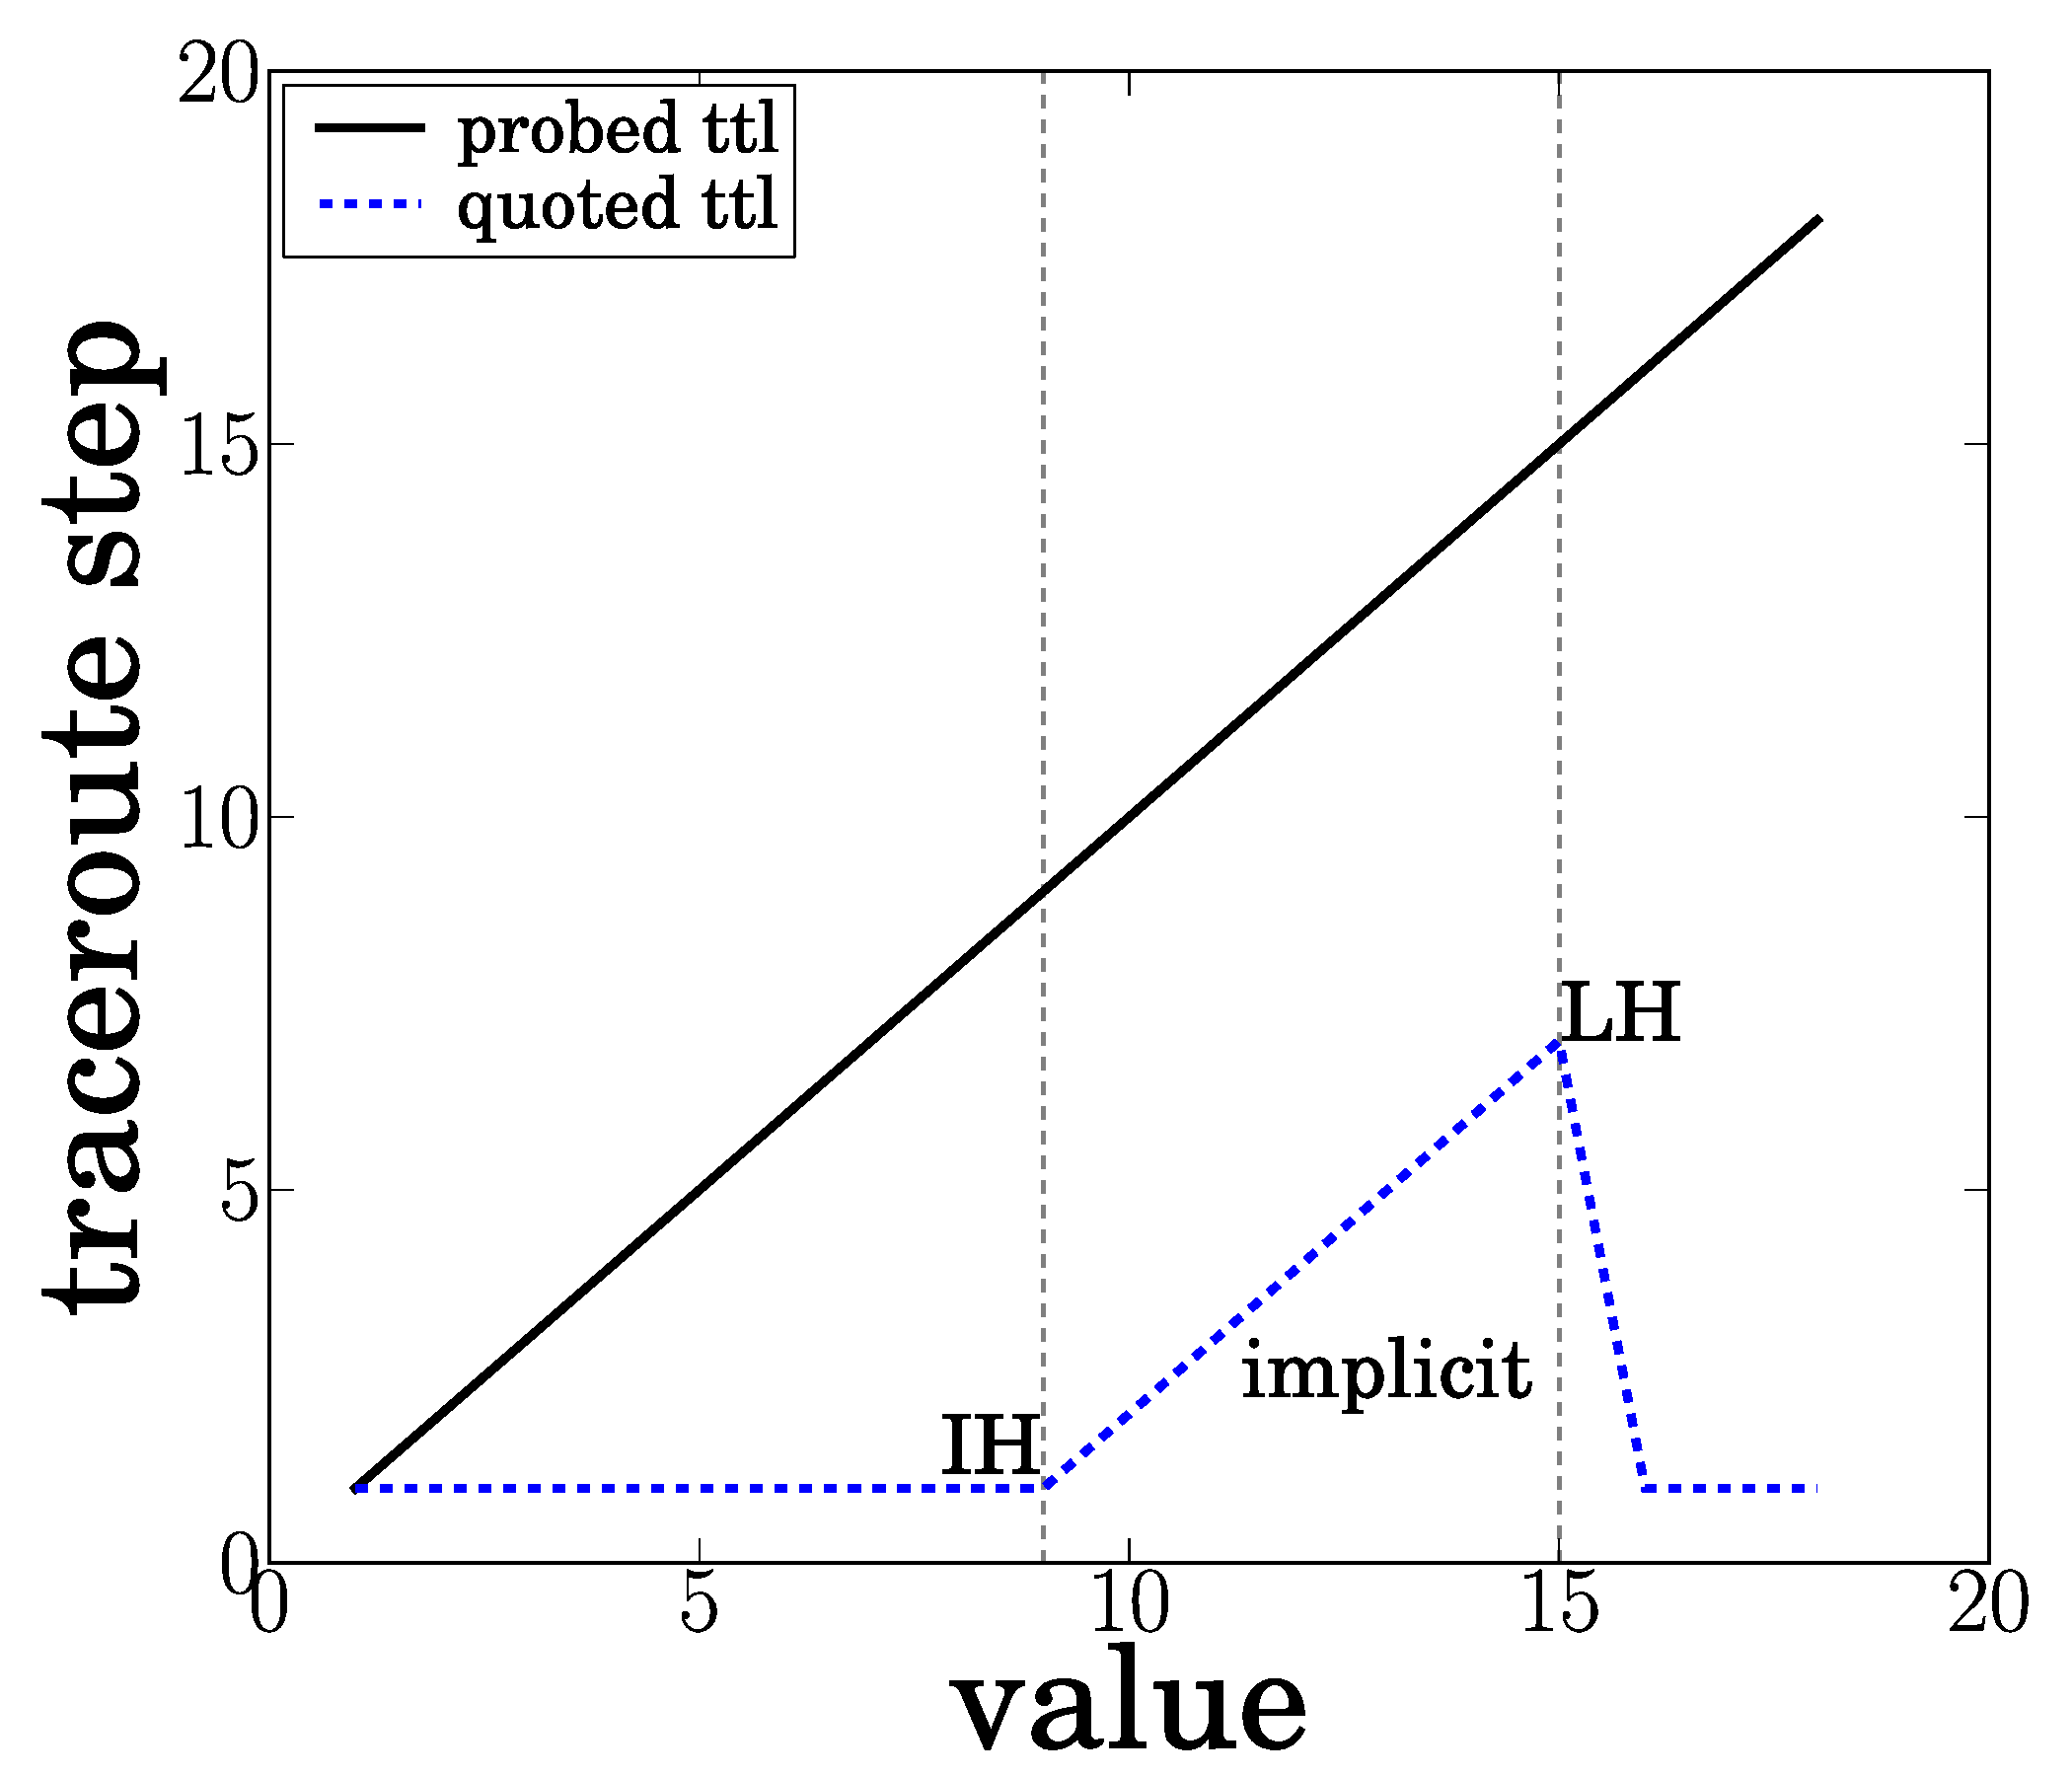
\includegraphics[width=4cm]{QuotedTTL}
  \end{center}
  \caption{Example of qTTL signature for an implicit MPLS tunnel.}
  \label{validation.qTTLFig}
\end{figure}

In this section we describe the used methodology to validate the MPLS signatures
used to reveal implicit MPLS tunnels (see Sec.~\ref{related.revealing}).
Basically, we compare the LSR position within an MPLS tunnel with the different
signatures values. Implicit tunnels are based either on qTTL or u-turn
signatures. Both of them are directly related with MPLS position \ed{unclear to
me what you mean by ``MPLS position''}.
First, the qTTL value refers to the IP-TTL of the \echorequest packet when it
enters the MPLS tunnel.  Therefore, a qTTL of $n$ in the resulting ICMP
\ttlexceeded means that the sent probe expired $n$ hops later than the Ingress
LER of the LSP, i.e., a LSR reply where qTTL$=n$ means that the LSR appears in
the \dfn{$n$-position} in the LSP.  This is illustrated in
Fig.~\ref{validation.qTTLFig}.  From the Ingress LER, the qTTL starts to grow
linearly with the LSP length.  We therefore expect observing a qTTL=$1$ on the
first LSR in the LSP, a qTTL$=2$ on the second LSR in the LSP, etc.  Second, a
u-turn value is related to the tunnel length, $L$, and the $n$-position of th
LSR within the tunnel (see Sec.~\ref{related.revealing}).

\begin{figure*}[!t]
  \begin{center}
    \subfigure[Tunnel length distribution]{\label{hist_length}
      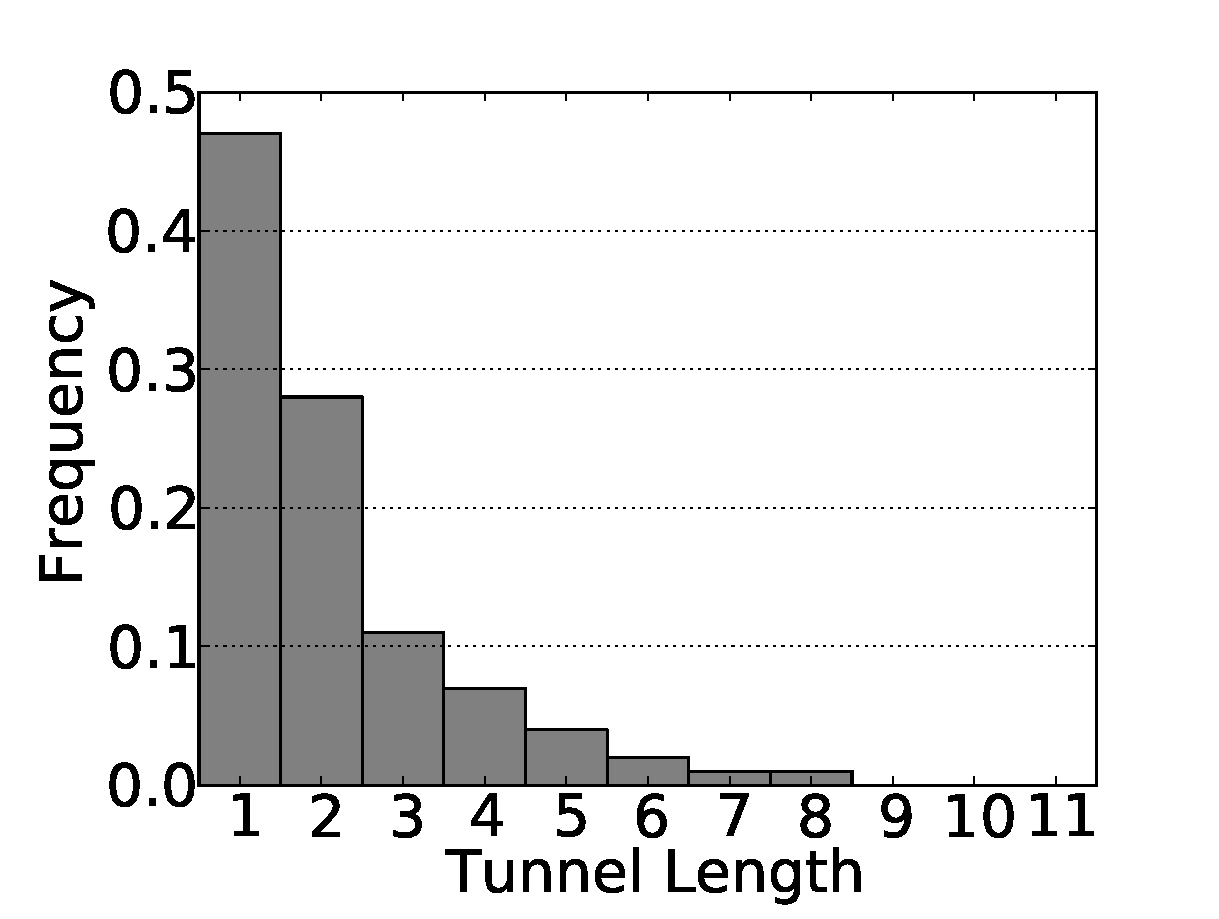
\includegraphics[width=4.3cm]{hist_length}}
    \subfigure[qTTL and $n$-position comparison]{\label{n_vs_qttl}
      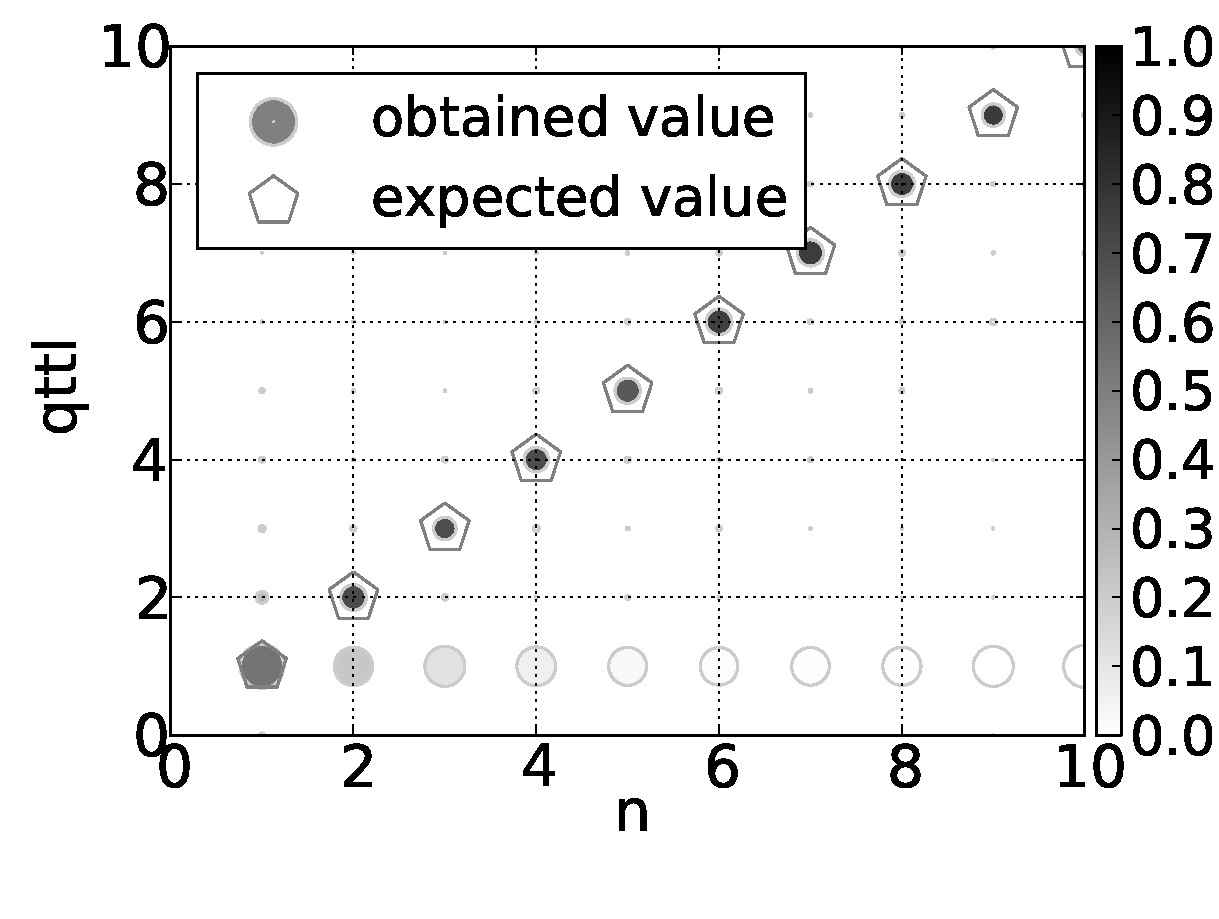
\includegraphics[width=4.3cm]{n_vs_qttl}}
    \subfigure[u-turn on LSRs revealed through RFC4950 and qTTL]{\label{fig_uturn_a}
      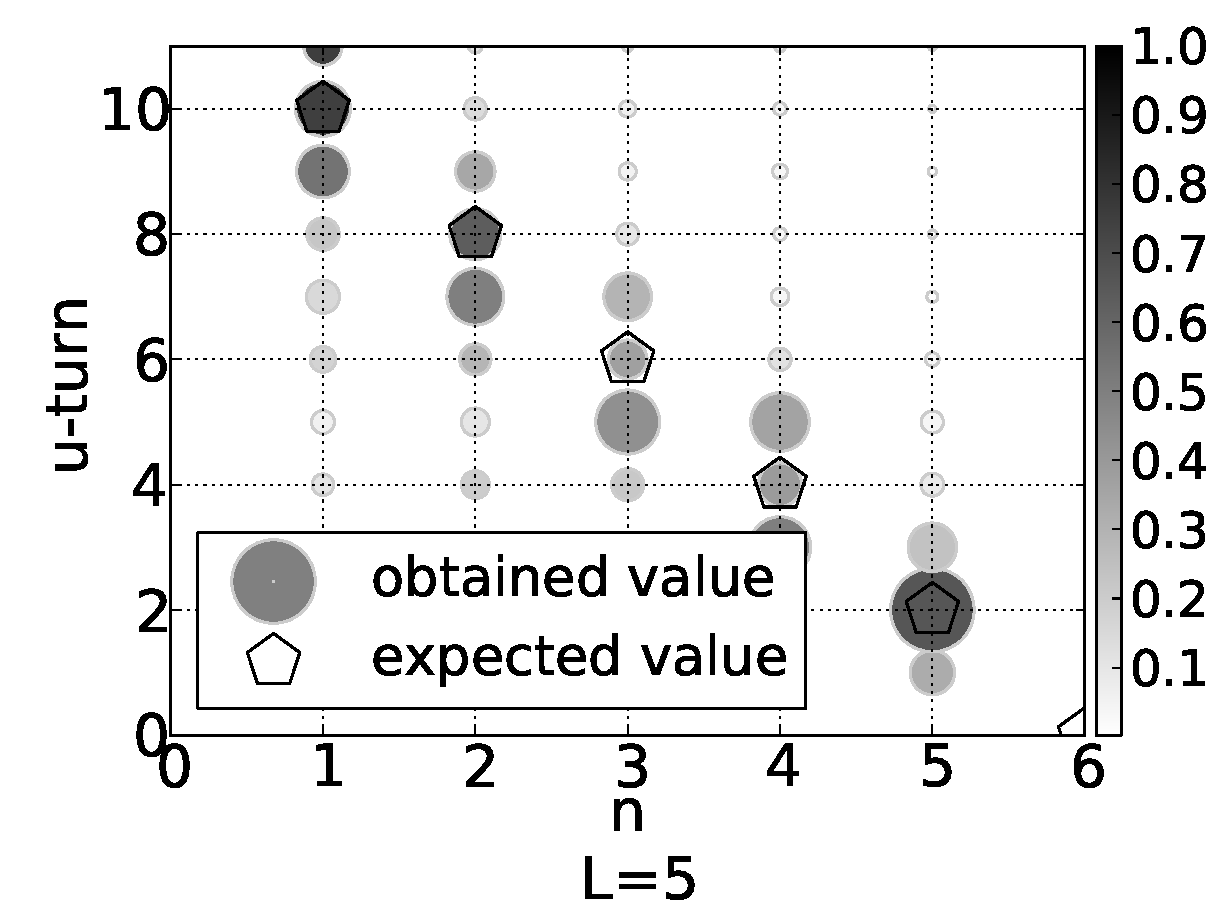
\includegraphics[width=4.3cm]{n_vs_uturn_L5_exp}}
      \hfil
    \subfigure[u-turn on LSRs where no other signature was found]{\label{fig_uturn_b}
      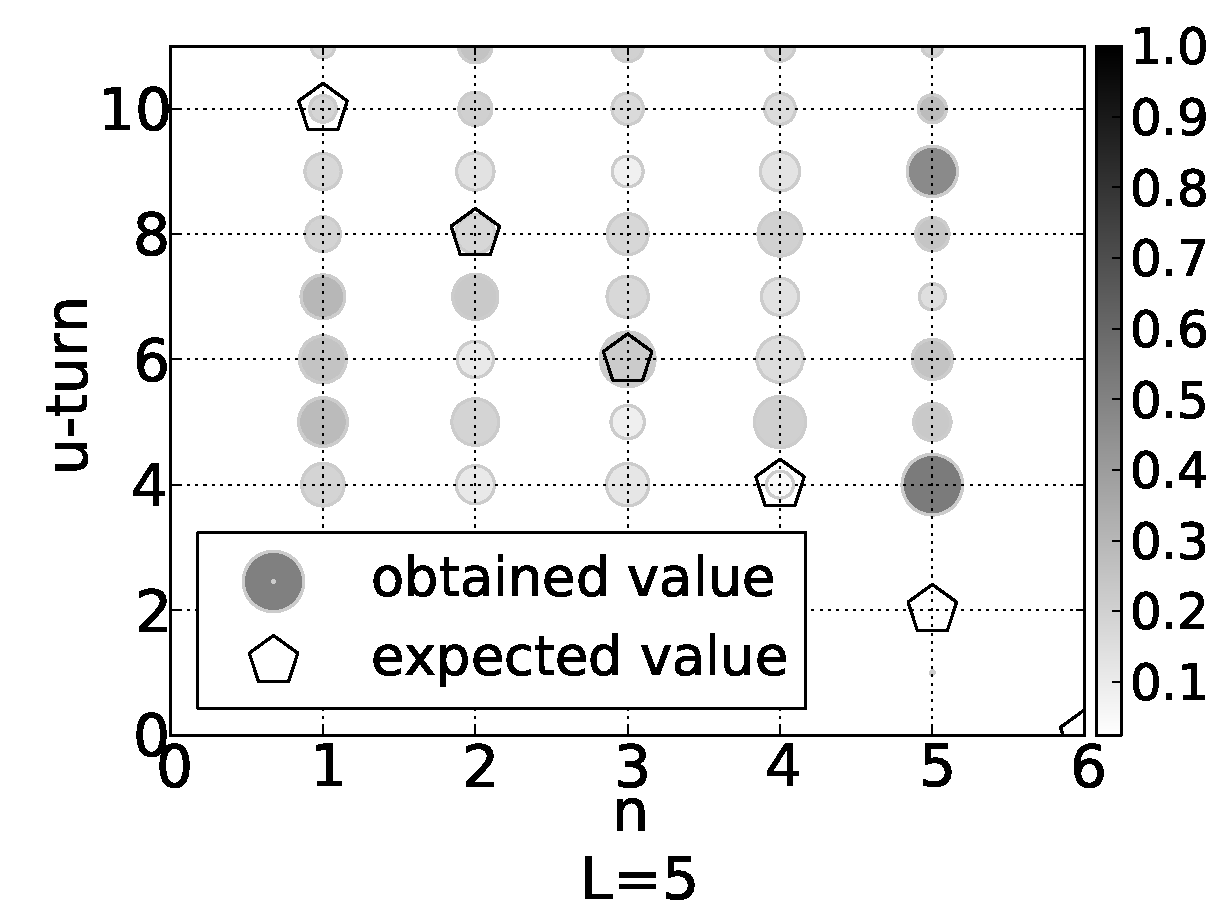
\includegraphics[width=4.3cm]{n_vs_uturn_L5}}
  \end{center}
  \caption{ Comparison between obtained and expected values for \textit{qTTL} and
  \textit{u-turn} signatures. On Fig.~\ref{n_vs_qttl},~\ref{fig_uturn_a},
  and~\ref{fig_uturn_b}, the circle size in the scatter plot is
  related with the occurrence frequency of Y-axis values regarding each
  $n$-position. The transparency of the circle is related with occurrence
  frequency of $n$-position regarding each Y-axis value.  For instance, on
  Fig.~\ref{n_vs_qttl} for values where $n>1$, the biggest circles are
  mainly located on qTTL$=1$ and qTTL$=n$ so this suggest that for a
  given $n$-position the qTTL value usually takes either the value of $1$ or
  $n$; in the same way, the transparency value suggests that for a given qTTL
  value the $n$-position usually takes the same qTTL value. 
  Fig.~\ref{fig_uturn_a} and~\ref{fig_uturn_b} suggest that u-turn value is
  overestimated.}
  \label{ig_signatures}
\end{figure*}


%\begin{figure*}[!t]
%\centering
%\subfloat[Case I]{\includegraphics[width=2.5in]{box}%
%\label{fig_first_case}}
%\hfil
%\subfloat[Case II]{\includegraphics[width=2.5in]{box}%
%\label{fig_second_case}}
%\caption{Simulation results for the network.}
%\label{fig_sim}
%\end{figure*}

Our signature validation relies on the hypothesis that the MPLS position matches
with the $n$-position  which an LSR is revealed by traceroute \ed{unclear}.
Indeed, we use a paris-traceroute~\cite{BRICE06}  based tool in order to assure
that probes follow the same path \ed{inconsistency here as you suggest later
that bias might be due to load balancing (not suppose to happen due to the use
of paris traceroute)}.
In order to validate our hypotheses, first, we compare a high reliable signature
such as \textit{qTTL} with  $n$-position, i.e., qTTL=n. The results are shown in
Fig.~\ref{n_vs_qttl} while Fig.~\ref{hist_length} shows the MPLS tunnel length
distribution \ed{how did you compute the tunnel length distribution?  Did you
include Ingress/Egress LER or not (i.e., L = Ingress + $|$LSP$|$ + Egress or L =
$|$LSP$|$)?}; which can help us to understand the number of LSR in each $n$
position.
We mainly notice that qTTL signature highly matches with $n$.
The bias $\textit{qTTL}=n \pm \vartriangle $ could occur due to two causes: one
is the limitation in our method to reveal the first LSRs \ed{1st LSR or Ingress
LER?} of the tunnel when RFC4950 is not implemented; and the second cause could
occur due to load balancers in the follow path \ed{follow path?}. In the later
case, the traceroute probes may follow paths with different lengths before
reaching the MPLS tunnel, yielding that the same qTTL value is revealed several
times in different $n$-positions. Fig.~\ref{n_vs_qttl} also shows that qTTL
frequently takes the value of $1$. This usually  means that \tpropagate is not
implemented \ed{we are not in the case of an implicit tunnel, so?}. However, we
found that around $2\%$ of LSRs do not react to qTTL signature, even if
\tpropagate option is activated, i.e., some LSRs interfaces located at $i_{n\pm
1}$ tunnel positions react properly to qTTL signatures but the LSR interface
located at $i_n$ position does not. However, $n$-position are highly reliable.
We found that in $58\%$ of the cases the $n$-position match with the qTTL value
while in $36,3\%$ of cases the qTTL signature is not present and takes the value
of $1$, and just $6,7\%$ of the cases presented have some bias around the
expected value $n$. This facts support our hypothesis: the  MPLS tunnel position
highly match with the $n$-position  which an LSR is revealed by traceroute.
Thereby,  we use $n$-position as a reference value to validate the u-turn
signatures.

The expected u-turn value is related with $n$ in the way
$\textit{u-turn}=2(L-(n-1))$, where $L$ is the tunnel length.
Because u-turn is commonly present in almost all LSRs, first, we compare $n$ vs
u-turn on LSRs  revealed either explicitly or qTTL based. Subsequently, we study
$n$ value on LSRs where u-turn was the only detected signature. We use the
filter $\textit{u-turn}>3$ to avoid false positives. The results for a given
tunnel length $L=5$ are showed on Fig.~\ref{fig_uturn_a} and
Fig.~\ref{fig_uturn_b}. Similar results was also obtained for other tunnel
length $L$ values. Basically, we noticed that the percentage of cases are close
to expected ones when the LSRs explicitly revealed  and qTTL is present
(Fig.~\ref{fig_uturn_a}). However on the set of LSRs revealed just by u-turn
signatures (Fig.~\ref{fig_uturn_b}) the cases commonly  does not match. If we
accept a bias of $ \pm 1$ around the expected value, we noticed that  on LSRs
explicitly revealed and qTTL signature based, the $60\%$ of obtained u-turn
signed cases match with the expected values. However, on LSRs revealed just
trough u-turn signature (therefore where it is really useful), the obtained
u-turn cases just match in $25\%$ with the expected value $2(L-(n-1))$.
Therefore, LSRs revealed through u-turn is highly inaccurate; mainly
because MPLS tunnels are not the only responsible on the variation in it length,
but also the load balancing is common for paths between the same pairs
source-destination \cite{BRICE07}. This issue is called \dfn{per-flow} load
balancing. Basically, packets that belongs to the same \dfn{flow} are treated
similarly \cite{BRICE06}. A flow is identified by the first 32 bits of
the IP \textit{payload}, e.g., TCP header. In the case of ICMP messages, this
fields refers to \texttt{Type}, \texttt{Code}, and \texttt{Checksum}.
By definition, u-turn signature is based on two kinds of ICMP messages:
ICMP \echoreply \texttt{Code 11} and ICMP \ttlexceeded \texttt{Code 0}.
Due to different codes for each ICMP message, there is no way to assure that
they belong to the same flow identifier and thereby to be sure that
u-turn value is caused just by MPLS tunnels.
